\subsection{Overall Performance and Skill Breakdown}
\label{sec:results}
\label{sec:skill-breakdown}

\begin{table*}[t]
\centering\small
\begin{tabular}{lrrrr}
\toprule
Model & No Skill & With Skill & $\Delta$ (points) & Failures (No/With)\\
\midrule
\inputtable{tables/combined_main.tex}
\bottomrule
\end{tabular}
\caption{Reference-relative scores on the unified 305-task inventory. All
tasks remain in each denominator; execution failures contribute zero. Pro No
Skill supplies the fixed references and is assigned the self-comparison value
50.00. GLM-5.3 is the retained augmentation result described in
Appendix~\ref{app:execution}. Differences use unrounded values.}
\label{tab:main}
\end{table*}

\paragraph{Procedural availability produces selective gains.}
Table~\ref{tab:main} covers 3,050 model--task--condition cells: 2,725
accepted judgments, 305 reference-self comparisons, and 20 execution failures.
GLM-5.3, GLM Flash, and Doubao improve by 0.45, 0.41, and 0.50 points with
Skill availability, whereas DeepSeek Flash and Pro decline by 1.19 and
0.25 points. The small aggregate changes motivate examining which educational
procedures help, whether agents access them, and what they ultimately deliver.
They do not support a uniform benefit from adding procedural resources.

\begin{figure*}[t]
\centering
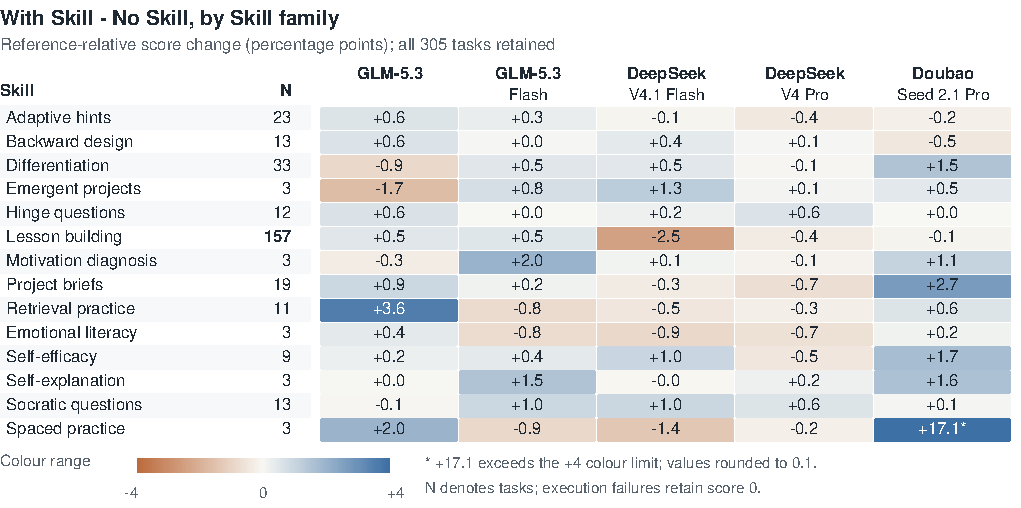
\includegraphics[width=\textwidth]{figures/skill_delta_v4.pdf}
\caption{With--No score differences for all five models across the 14 Skills.
Each cell retains all tasks in its family, including failures; $n$ gives the
family size. Color saturates at $\pm4$ points; labels show rounded
differences. Complete means and failure counts appear in
Appendix~\ref{app:inventory}.}
\label{fig:skill-breakdown}
\end{figure*}

\paragraph{Different procedures reveal different strengths.}
Figure~\ref{fig:skill-breakdown} groups the same accepted scores by designated
Skill, without changing the judge or task membership. GLM-5.3, GLM Flash,
DeepSeek Flash, Pro, and Doubao have positive differences on 10, 11, 7, 5,
and 11 of 14 families. For example, GLM Flash gains 0.95 points on Socratic
questioning but loses 0.81 on retrieval practice. DeepSeek Flash gains 1.01
on self-efficacy support and 0.98 on Socratic questioning, yet loses 2.49 on
lesson building. These contrasts locate procedure-specific opportunities
that the overall mean conceals.

\paragraph{Coverage and completion explain part of the variation.}
Lesson building contributes 157/305 tasks (51.48\%), while five families
contain three tasks each. Its decline contributes $-1.28$ points to DeepSeek
Flash's overall $-1.19$ change. Equal weighting of the 14 families instead
gives changes of $+0.47$, $+0.34$, $-0.09$, $-0.13$, and $+1.87$ points
in the model order above; this diagnostic describes coverage sensitivity,
while the task-weighted mean remains primary.

Completion also matters. Doubao's spaced-practice gain is $+17.06$ on three
tasks, including one failed No Skill execution; the two pairs completed in
both conditions differ by only $+0.59$. Across all common-valid pairs, the
four native-access models change by $+0.25$, $-0.54$, $-0.09$, and $+0.36$
points, respectively. DeepSeek Flash's decline therefore persists after
conditioning on completion. Appendix~\ref{app:inventory} supplies family
denominators and failure diagnostics. These single-run differences describe
the retained executions; they do not establish significance across model
or judge resampling.
